%
% ewsn-full.tex
%

%
% NOTE
%
% ewsn-proc is based on sigplan-proc-varsize 
% The default of sigplan-proc-varsize is 9pt, indented paragraphs (ACM style)
% For EWSN or other 10pt conference, use the 10pt option
\documentclass[10pt,nocopyrightspace]{ewsn-proc}

% TODO do we really need this?
% % hack to avoid the ugly ACM paragraph definition
% % => can't leave blank line after this
% (remove comment for this hack)
% \renewcommand{\paragraph}[1]{\vskip 6pt\noindent\textbf{#1 }}

\usepackage{graphicx}
\usepackage{balance}
\usepackage{comment}
\usepackage{xurl}

%
% NOTE
%
% The EWSN reviewing process is double blind: authors must not
% reveal their identities to the reviewers. Names and affiliations
% will only be added for the camera-ready version (see below)
%\numberofauthors{1}
%\author{
%\alignauthor Double Blind \\
%  \affaddr{do not reveal authors}
%}


%
% NOTE
%
% The command \alignauthor (no curly braces needed) should
% precede each author name, affiliation/snail-mail address and
% e-mail address. Additionally, tag each line of
% affiliation/address with \affaddr, and tag the
%% e-mail address with \email.
\numberofauthors{1}
\author{
\alignauthor Pēteris Račinskis \\
    \affaddr{University of Latvia}\\
    \email{pr13001@edu.lu.lv}
}


\title{Sensor Node Design for Forest Trail Visitor Load Estimation}


\begin{document}

\maketitle

\begin{abstract}
TODO

TODO 

TODO

TODO

TODO

TODO

TODO 

TODO

TODO

TODO

TODO

TODO 

TODO

TODO

TODO

TODO

TODO 

TODO

TODO

TODO

\end{abstract}

%
% NOTE
%
% Do not provide category, terms, keywords for the reviewed submission.
% They will only be added for the camera-ready version. Instructions will
% be provided for the camera ready version.

%
% A category with the (minimum) three required fields
% \category{H.4}{Information Systems Applications}{Miscellaneous}
%A category including the fourth, optional field follows...
% \category{D.2.8}{Software Engineering}{Metrics}[complexity measures, performance measures]
% \terms{Delphi theory}
% \keywords{ACM proceedings, \LaTeX, text tagging}

\section{Introduction}
Latvia is a nation proud of its extensive forest cover, and various sights located in forested surroundings account for a significant fraction of stopping places frequented by any tourist deigning to venture outside the major cities. As in any other visitor-oriented industry, having a clear understanding of attendance patterns is very important for the management, maintenance and adequate monetization of destinations for the management of nature tourism destinations. The very qualities that make these locations desirable in the eyes of potential visitors - remoteness, limited marks of human presence, untouched natural scenery - naturally create a series of challenges when it comes to creating data collection infrastructure. While under normal circumstances this might be enough to thoroughly dissuade any further efforts, events such as the recent (and as of the writing of this paper, still ongoing) COVID-19 pandemic show that traditional methods of visitor count estimation might not be adequate in keeping up with changes in travel patterns. With the shutdown of international travel and various social distancing measures in place, domestic nature tourism sites have experienced damage\cite{TrailDestruct} and full-on closures\cite{TrailClose}. Traditional methods of estimating how many sightseers have walked a trail and used its amenities include surveys and short-term targeted data collection, but these are not adequate for tracking both the long-term evolution and short term fluctuations in load. The negative effects of this lack of information can range from inadequate or out-of-service trail facilities, over- or under-investment in certain objects, unnoticed obstructions, wildlife destruction off-path and lost business opportunities.

Thankfully, over the past decade significant progress has been made in the development of low-power, long-range communications technology that enables relatively inexpensive data collection even over large areas in difficult terrain. Coupled with inexpensive sensor and computing hardware these advances make possible persistent data collection of the kind and scope required for visitor count estimation. The goal of this paper is to propose a specific architecture for a wireless sensor node that might be used to this end, using LoRa and PIR technology.


\section{Related Work}

Naturally, this being a rather mundane problem, efforts have been directed towards solving it before. One of the more prominent papers on the subject, \textit{“Estimating visitor use at attraction sites and trailheads in Yosemite National Park using automated visitor counters”} by Pettebone et al.\cite{Pettebone:Yosemite}, takes the relatively straightforward approach of utilizing commercial off-the-shelf (hereafter COTS) wildlife monitoring equipment without any networked communication capability to count visitors in select locations across the park. Most of the paper is devoted to cross-referencing the data collected in this fashion with observations through other methods and verifying its reliability. The devices used in the paper are rather bulky and expensive, using active infrared technology to detect interruption events between a beam source and sink. \textit{“Methods for Visitor Monitoring in Recreational and Protected Areas:
An Overview”} by Muhar et al. \cite{Muhar:Methods} compares electronic counting methods to alternatives and notes the extensive calibration times required for sensors using photoelectric detection methods in practice. 

For more geographically proximate takes on the subject one can turn to \textit{“Visitor monitoring in nature areas – a manual based on experiences from the Nordic and Baltic countries”} by Kajala et al. \cite{Kajala:Baltic} and \textit{“Visitor Monitoring Guidelines in Protected Nature Areas; Example: Slītere National Park, Latvia”} by Smaļinskis et al. \cite{Slitere}. Rather than academic articles, these publications follow a longer form approach of examining the problems faced by park management when attempting to implement visitor count estimation systems, offering solutions, explaining the tradeoffs between them, as well as suggesting various tips and pitfalls to avoid. An interesting observation made in both of these, which seems to be less acknowledged further abroad, is the ever-present risk of vandalism and sabotage by park-goers; any equipment that has an obviously technological appearance stands at risk of being destroyed for no particular reason, and care must be taken to make any such device as inconspicuous or inaccessible for casual sabotage attempts as possible.

Finally, it needs to be acknowledged that for any application exploitable by reasonably mature technologies, commercial solutions are bound to exist. EcoCounter is a company that offers integrated sensor-node and data collection service solutions \cite{EcoCounter}. These utilize PIR detection technology and cellular networking, the latter of which combined with the turn-key service-based approach make competition on price and application freedom viable.
 

\begin{figure}[t!]
\centering
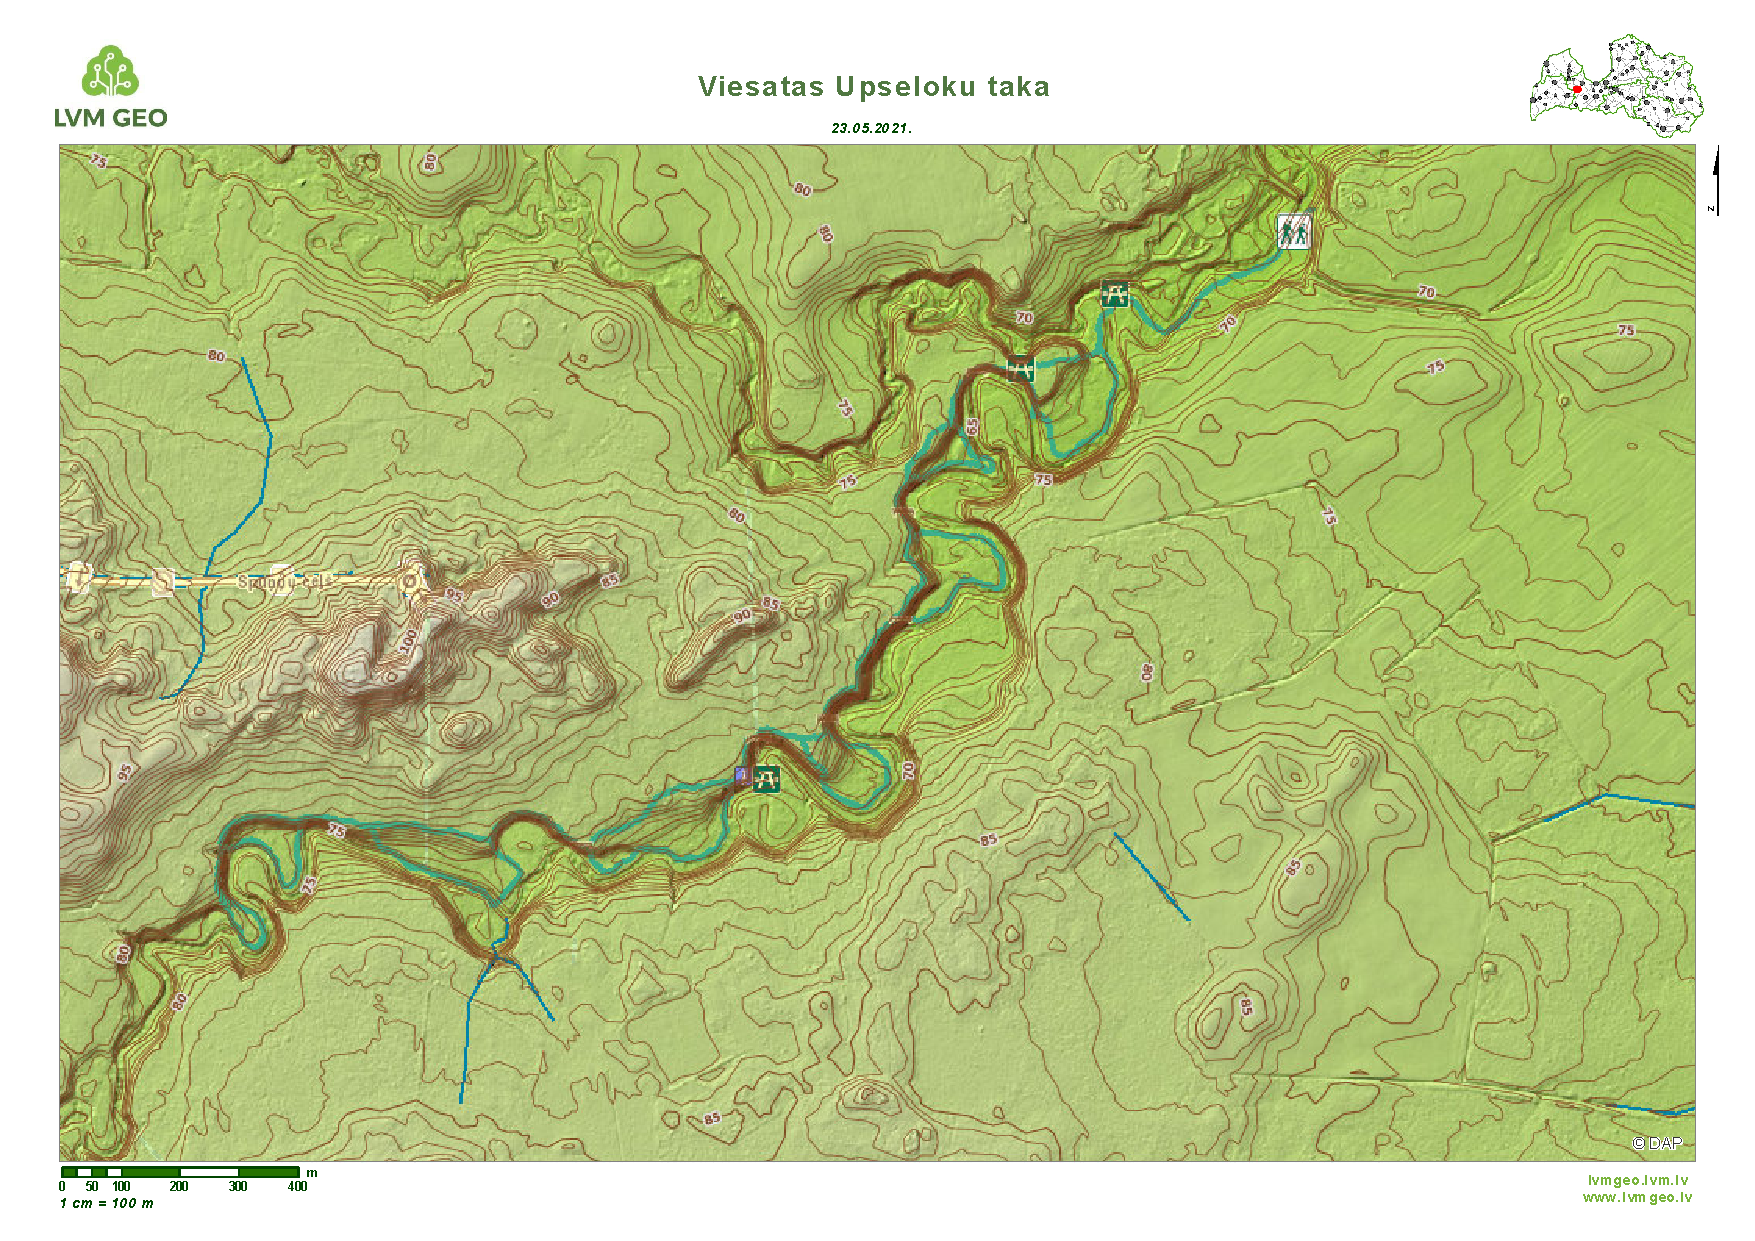
\includegraphics[height=2.2in]{./Images/map1-Viesata}
	\caption{Topographical map of the Viesata River Bends trail, one of the more challenging locations for WSN application. Much of the trail follows the prominent ravine carved by the flow of the river, the banks of which are sheer inclines up to around 10 meters in height and covered in dense vegetation. Straight-line distance between park entry and the furthest point on the track is around 2.1km, and it follows the straight-line/loop pattern. \textit{Map generated using the LVM Geo tool courtesy of AS "Latvijas Valsts Meži"}}
\end{figure}

\begin{figure}[t!]
\centering
\includegraphics[height=2.2in]{./Images/viesata_image}
	\caption{Photo of the Viesata Ravine, taken looking from around the mid-point of the River Bends trail towards the entry point and parking lot area. While for much of its length the trail follows the edge of the embankment, at several points it descends into the gully below, where line of sight is obstructed by terrain in addition to vegetation - and it is precisely there that many points of interest are located. \textit{Photo by author}}
\end{figure}


\section{Motivating Application}

The idea for the project undertaken and described herein was originally provided by AS “Latvijas Valsts Meži” (hereafter referred to as LVM) staff. For the reasons described before, managing and tracking visitor loads has become a problem of interest for management teams responsible for operating the large number of tourism objects owned by the company, predominantly in densely forested areas. As such a number of locations were visited and surveyed by the author to determine constraints and requirements for any WSN system to be deployed in these settings.

\begin{itemize}
\item \textbf{Tervete.} A small town southwest of Jelgava surrounded by LVM-owned and operated properties. A popular tourist destination and home to a dense network of interconnected forest trails criss-crossing the hilly terrain and reaching out in all directions from the town.
\item \textbf{Viesata River Bends.} Located approximately half-way between Jaunpils and Tukums, a mostly linear system of tracks following the river Viesata as it carves a rapid series of steep bends through the elevated plain surrounding it. Features a main path tracing the top of the embankment with branching detours descending down towards the river where various wildlife-related objects of interest are to be found.
\item \textbf{Kartavkalns.} Not far from the Viesata trails, a more man-made destination. Centered around the remains and partial reconstruction of an ancient hill-top fort, this locality is dominated by a central elevated location and paths descending its slopes on all sides.
\item \textbf{Vilce.} Almost on the Lithuanian border, a meadow situated at the confluence of three shallow ravines and surrounded by forest in all directions.
\end{itemize}

All taken together, these four locales form a relatively representative sample of the topographical conditions and layouts one can expect to find at LVM forest trails. Distinct types of compact (a single central location with trails stretching out radially and along concentric trajectories, conserving straight-line distance) and looped (extending in a single direction from the entry point for a long way) trails emerge. Additionally, some locations might host several objects - Tervete can be viewed as having several distinct trails that fall into one of these categories. 

Compact style layouts are more common, and enforce less exacting requirements on the sensor network. Even though the total length of walkable trail and number of monitored locations might be higher, the straight-line distances tend to be shorter, placing less vegetation and fewer potential terrain obstructions between the node and a base station (if one is required by the system architecture). Therefore the limiting use case comes in the form of looped trails, such as Viesata Bends - which will be used as the motivating application. On-site examination revealed the following challenges:

\begin{itemize}
\item \textbf{Range.} Some of the longest straight-line distances found among the localities surveyed at around 2.1km. Impose limitations on viable network technologies straight away. 
\item \textbf{Uneven terrain.} Though large undulations in terrain are relatively rare in Latvia, with flat plains or gently sloping hills dominating most of the landscape, the steep if shallow ravine serves as a reminder that line of sight considerations must still be taken into account even at relatively short ranges. Furthermore, while a reflected signal path can be considered viable in some circumstances, the repeated curves of the gully mean multiple reflections (along with the corresponding signal attenuation) would be required..
\item \textbf{Dense vegetation.} Rather unsurprisingly, even where the signal path is not impeded by the ground, it must pass through dense forest.
\item \textbf{Conspicuous sensor location.} The forest floor is in many cases not covered by any form of grass or shrub, with only sheer tree trunks lining the sides of footpaths. Remembering the aforementioned concerns about vandalism, care must be taken to make the sensor nod as inconspicuous or inaccessible as possible. Remote sensing methods or compact detection devices are therefore preferable.
\item \textbf{Patchy reception.} Although hardly a scientific test, moving further along the trail and especially down into the ravine results in observable decay and even interruptions in cellular network reception.
\end{itemize}

\section{Approach}
The visitor counting problem can be broken down into two main components: visitor detection and sensor network design. In the case of most proposed network architectures and visitor detection schemes, the problems can be tackled independently, as the practical upshot of their employment is the same regardless.

\subsection{Visitor Detection}

In addition to the author’s original idea of using the RF signature of nowadays ever-present cellular phones as a clear marker of human presence in an otherwise low-radiation forest environment, a range of possibilities were suggested by the professor, class and others consulted by the author. Discussion with trail staff revealed a strong preference for technologies which do not require any kind of digging or other type of disruption to the surrounding environment, with low-intrusion devices attached to trees or freely standing on the ground being seen as the optimum form factor - thus disqualifying induction-sensing ground loops and buried pressure pads. The following approaches were considered for person detection, each of which is discussed in more detail below:
\begin{itemize}
\item Active IR
\item Passive IR
\item Ultrasonic Reflection
\item Audio Signature Detection
\item RF Signature Detection
\end{itemize}


\subsubsection{Active IR}
Also known as a light barrier, this is one of the oldest, most straightforward and widely used methods for detecting the presence or absence of objects in space. Examples of this technology can be found in a wide range of applications, ranging from consumer electronics to building automation, security and alarm equipment, to industrial automation where these devices are ubiquitous as position references and presence indicators.

Active IR relies on a radiation source and detector, either in two separate devices on either side of a gap where an object is expected to appear, or in one location with a reflector on the other side. The sensor registers a change of state when the beam is broken. This is the detection method employed by the commercial off-the-shelf wildlife tracking instrumentation in the Yosemite system\cite{Pettebone:Yosemite} as well as some case studies mentioned in the Baltic-Nordic manual\cite{Kajala:Baltic}. Given the two-sensor or sensor-reflector setup, a notable concern is the alignment of the devices, without which detection is impossible. This requirement also makes it more difficult to make the solution sabotage-resistant, as the paired setup is more easily noticed by passers-by, and more easily rendered inoperational.

Alternatively, reflectorless designs are possible where the opposite is the case - a low baseline return is assumed and the sensor goes active in response to the light reflected from a nearby body. This does away with any alignment requirements but results in significantly reduced detection ranges. This type of setup is also more difficult to calibrate, as one has to contend with the broad range of possible surface reflectivities, surrounding stationary objects and continually changing ambient lighting conditions, all of which complicate setting decision thresholds.

The radiation may in either case be continuous or pulsed, the latter case allowing for fast, transient interruptions to be filtered through the use of impulse counting. As it has to constantly emit radiation in addition to powering the light detection circuitry, an active IR solution can generally be assumed to have higher constant current draw (by a figure on the order of at least 10mA, as elaborated upon in efforts to design active IR detector hardware \cite{ActiveIR}).


A related family of technologies employs the same principle but with different types of radiation - such as radio-frequency or laser light. Both of the above improve system range at the expense of system cost and power consumption. The use of RF barrier-type detectors is described in the Slitere case study paper\cite{Slitere}.

\subsubsection{Passive IR}
Where active IR is the go-to solution for detecting the presence of moving objects at particular locations, Passive IR (PIR) can be said to be the same for simple motion detection applications. Mostprominently featured in alarm systems and automatic lighting, this technology does away with the transmitter half of the equation and relies on the temperature differential between the background and a typical moving object of interest (person, animal or vehicle) instead.

A typical PIR motion detector uses a pair of pyroelectric crystals with radiation from slightly different fields of view focused on them through fresnel lenses, with a voltage differential across these triggering the output. Being a passive device, the power consumption of a PIR detector can be remarkably low - an example application by Texas Instruments discussed in two technical manuals\cite{TI:PIR}\cite{TI:APP} shows current consumption in the single-microamp range when only the motion detector is active. This is an improvement over any design using an actively radiating element by several orders of magnitude.

The tradeoff, however, as discussed in Kajala et al.\cite{Kajala:Baltic}, is reduced sensing accuracy, in some sense similar to the tradeoffs incurred in the transmitter-less active design. PIR is more susceptible to environmental false positives, as well as changes in ambient conditions such as lighting and weather effects (fog, etc).

Quite notably this is exactly the approach favored by Eco-Counter, a manufacturer of people-counting devices and turn-key solutions for use in both urban and rural/wildlife environments.

\subsubsection{Ultrasonic Reflection}
An alternative to reflector-less active IR or PIR motion detection using ultrasonic transducers. Fairly popular as a search engine result and in hobbyist electronics circles, yet does not offer any discernible advantages over light-based methods, all the while demanding greater operating currents and bulkier form-factor devices. 

\subsubsection{Audio Signature Detection}
While the forest is a naturally noisy environment, humans tend to produce two highly distinctive types of audio signals when present - voices and footsteps. In principle these could be used to indicate the presence of a visitor or group thereof, and detecting them is trivial with access to sufficient signal processing power.

Voice detection is probably the hardest of the two problems, but also the one with by far the most potential commercial applications - thus ample funding and development time has been invested in various types of COTS systems that can accomplish this objective, mostly for use with voice commands in consumer electronics. A typical approach might consist of a loudness threshold detector and a voice recognition IC such as the HM2007\cite{HM2007} that can recognize certain words or phrases. In 2021 especially it should be possible to quite reliably discriminate the features of a human voice from ambient noise. 

However, most of this work seems to have gone into short-ranged consumer goods designed for use in relatively silent rooms. Using ambient noise levels to switch relatively high-powered DSP circuitry on or off may be a strategy well suited for an indoors environment, but seems far less applicable to the forest environment. Moreover, the author’s own experiences while surveying the sites suggest that most of the time visitors are either silent or talking at rather low volumes, which makes voice an extremely unreliable indicator of presence.

The other method proposed is footstep detection. Being the only species of animal to walk upright, wearing hard-soled footwear to boot, humans produce a unique auditory signature when in motion. Furthermore, this is our preferred method of locomotion, which means that one can reliably count on detecting its signature whenever moving humans are around. The fundamental idea of isolating both the low-to-ultrasonic frequency spectra of single footsteps as well as their predictably repeating pattern has been studied for military applications\cite{NATOfootsteps}, and found to be a viable direction of inquiry. As per the cited source, signatures significantly above the noise floor can be extracted in the 100-300Hz as well as 25-26kHz ranges. Additional work still needs to be done in learning to robustly isolate these from other possible sources of noise in these ranges, but one can expect the periodic step pattern to make this task drastically easier than it would appear at first glance. 

A notable advantage a sound signature based detection system could offer over the previously examined ones is the lack of positional/directional coupling with the path of travel - the sensor can be more easily concealed away from the trail, in more favorable environmental and RF communication conditions - such as high in trees or off-trail.

\subsubsection{RF Signature Detection}
The original idea that inspired this paper, yet turned out to be impossible to test in practice due to a delayed SDR module which was to be used to test the RF emissions of typical cellular devices under various practical conditions. A trail in the forest is far removed from most sources of EMI that can be found in densely populated or industrialized areas, which makes the phone carried by nearly all of us everywhere we go a strong indicator of human presence. Furthermore, the sources of interference that are present away from human-settled areas can be expected to be of highly chaotic nature and cover broad frequency bands, which should prove easily distinguishable from structured narrowband communications transmissions.

As with audio signature detection, the same advantages apply - there are no directional elements and the device can be placed safely away from the track itself.
 

\subsubsection{Selected Method}
Having taken all of the above considerations into account, it was decided that in order to accomplish the goal of producing a system design that can be implemented in reality given some time and funding, as well as a working proof-of-concept prototype of the sensor node, the most viable approach is \textbf{PIR motion detection}. The reasons can be summed up as follows:
\begin{itemize}
\item \textbf{Availability.} As of writing this, the world is still gripped by a global pandemic, which has placed a heavy strain on international supply chains. Components which would have arrived from manufacturers in East Asia in under 2 weeks just two years ago can now take much longer to arrive. Planning around these constraints is difficult given the relatively short time frames available for carrying out single-semester university projects. PIR devices are extremely common and readily available for prototyping use even from local suppliers.
\item \textbf{Simplicity.} Compared to footstep signature detection, which also made the shortlist, this is a mature and well-understood technology, which can be integrated into a board design straight off a reference manual, and produce a straightforward discrete ON-OFF value for the controller. Whereas footstep detection might not even be possible to reduce to analog electronics - while in the ideal case of perfectly sinusoidal baseband and signature waveforms this problem reduces to two-level amplitude shift keying, in practice the system needs to account for the distinctive and varied patterns that could be found in different individuals’ gaits on different surfaces, under different conditions. This might not be possible without additional digital signal processing, and is in any case a problem that requires significant amounts of further work.
\item \textbf{Low Power Consumption.} The single-figure microamp current draw figures possible for PIR motion detectors are a hard proposition to beat. 
\end{itemize}


\subsection{Wireless Network}
The second half of the wireless sensor network is the communication network itself. An architecture must be chosen which can accommodate the required data throughput rates under the environmental conditions related to the application. In this case, the key requirements can be summed up as follows:
\begin{itemize}
\item \textbf{Throughput.} Counting visitors requires only small amounts of transmitted data - essentially just a timestamp for each recorded event - and even the largest deployments aren’t expected to consist of more than a few dozen sensor nodes. Almost any wireless network architecture on the market will be able to meet these throughput requirements.
\item \textbf{Latency.} As with throughput, latency is largely irrelevant. A node would generally only need to transmit information a few times a day, and the collected data is not intended to be used for any real-time control purposes.
\item \textbf{Reliability.} Low error rates are important, but zero error rates are not a requirement. The network should be tolerant to environmental factors, but the intended statistical aggregation of the collected data, low node counts and mostly RFI-free surroundings with the consequent low collision probabilities mean that a small packet loss probability is acceptable, especially when data retransmission schemes can be implemented.
\item \textbf{Range.} By far the dominant consideration. Assuming a central collection hub, distances between it and the farthest nodes can range up to several kilometers (2100m in the example studied above), with substantial amounts of dense vegetation and possibly undulating terrain in-between. 
\item \textbf{Power usage.} The most important consideration after communication range. In order for the sensor network to be viable from a business perspective, service expenses need to be kept down, which means frequent battery changes/recharges should be avoided at all cost. 
\end{itemize}

\subsubsection{Type Selection}
When it comes to selecting a WSN architecture, it usually comes down to a choice between the three most common categories of solution - low-power personal area networks (LoWPANs), low-power wide area networks (LPWANs) or reliance on existing cellular infrastructure.

\textbf{Cellular networks} are present in and around most populated areas, offer high reliability, high throughput communications even at relatively long ranges and a mature, well-understood technological base to work with. Almost invariably, however, this comes with a power consumption penalty. Moreover, due to the restricted, subscription-based service provision model, operating such a network incurs a cost overhead. Surveying the locations mentioned in the problem description reveals that access to cellular networks is available at all of them, and in 2021 a major Latvian mobile carrier such as \textit{Latvijas Mobilais Telefons} is able to claim at least  some level of reception almost everywhere in the country. As such it comes as no surprise that this technology is used in the COTS visitor counting solutions offered by the aforementioned \textit{Eco-Counter}.

\textbf{LoWPANs}, typically operating on physical layers such as the IEEE 802.15.4 protocol specification, are generally optimized for short ( $<$ 200m ) transmission distances and scale by forming mesh networks - where every node serves as a router and packet forwarder. This approach is favorable when the nodes can be expected to be relatively densely packed and uniformly distributed, with no distant outliers - a condition which cannot be guaranteed under the problem specification given above. A more congested network where nodes also function as routers results in an energy overhead for communication that isn’t strictly necessary unless throughput requirements mandate it.

\textbf{LPWANs} emphasize very low power requirements almost to the exclusion of all other criteria. As of 2021, there are 3 major contenders in this market niche, all proprietary technologies, whose advantages and disadvantages, discussed in Mekki et al. \cite{LPWAN-compare}, as they pertain to the visitor counting problem can be summed up as follows:
\begin{itemize}
\item \textbf{Sigfox.} A very long range (up to 40km), extremely low throughput (100bps, limited to 140 messages-day) ultra-narrow bandwidth (100Hz at 868/915/433MHz) ISM band technology. Not an international standard - developed by a single company. Limited support for bi-directional communications. Meets the range and power requirements by sacrificing heavily in data rates, which matter little for this specific use case. 
\item \textbf{LoRaWAN.} Long range (up to 20km under ideal conditions), variable throughput (up to 50kpbs, much lower under most configurations) ISM band technology. The physical layer of the standard relies on a proprietary chirp spread spectrum modulation technique that has been reliably reverse engineered in Knight et al. \cite{Lora-decode}, which enables reception below the “noise floor” - negative signal-to-noise ratios \cite{Lora-docs}. Relatively high data rates can be maintained at long ranges while maintaining relatively low transmitter power. Standardized by the LoRa-Alliance, implementations available from many vendors internationally with a growing support base in software and hardware. Meets the range requirements assuming it is possible to correct for local variation in reception\footnote{While under ideal conditions\cite{LORAWAN-optimal} ranges of 15-30km can be attained, when faced with vegetation and hilly terrain communication can be disrupted even at short ranges\cite{LORAWAN-hills}}, this is the middle-of-the-road option in most aspects, and the most well-documented one.
\item \textbf{NB-IoT.} Medium-to-long range (up to 10km) relatively high throughput (200kbps) system based on LTE and operating in licensed frequency bands. As the shortest range, highest power and costliest this is also the least desirable option.
\end{itemize}

\textbf{Selection.} After taking the above factors into consideration, LoRaWAN has been selected as the network technology for this project. Cellular networking is attractive due to ready availability of pre-existing infrastructure, but a major drawback is high power consumption - cellular transmitters operating at maximum ranges may have to consume thousands of milliwatts of power as opposed to the 20mW transmit power limit of LoRa transceivers. \cite{Lora-docs} Moreover, COTS systems utilizing it already exist - therefore limiting the possibility of innovation in this direction and opening up opportunities for competition on cost by using a more lightweight, less power-hungry technology for the individual sensor nodes. 

Since the environment is covered in both thick vegetation and uneven terrain, care must be taken in the design process to compensate for the shortcomings of the selected technology in these circumstances - as empirical studies have found\cite{LORAWAN-hills} that both can create deadzones and significantly impair RSSI.


\section{Design}

\subsection{Scope}
A complete sensor network solution requires the sensing elements, transmitters, some form of collector or aggregator, and a data storage and presentation backend. In order to actually implement the system all of these elements would have to be provided and operational. Given the early stage of the development process, time and resource limitations, however, the scope of this particular project has been limited to only the sensor node itself. This includes the visitor detection and wireless data transmission stages of the information pipeline. Such a choice was made primarily because the viability of the data collection method itself is what determines whether a need even exists for the substantially more time- and resource- intensive base station design. Physical implementation and in situ testing would be required to determine this, and during the prototyping and small scale initial deployment phases a COTS base station can be used, even at considerable unit cost premium.


\subsection{Hardware}


\subsubsection{Overall}
In the process of sensor node hardware development it was quickly realized that the control-transmission and motion event detection subsystems are largely independent and only linked through a narrow interface of common power supply potentials and 1-2 discrete-valued data lines. Furthermore, these modules are subject to some diametrically opposed design incentives:

\begin{itemize}
\item The detector needs to be located low to the ground and near the trail in order to be effective. The best positions for the sensor are unlikely to coincide with the points where transmission losses are minimal.  It also needs to be as small and unobtrusive as possible.
\item The transmitter needs to be located as high up in the forest canopy as possible to minimize direct line of sight obstruction as a consequence of both terrain and vegetation. It also needs to house an antenna that minimizes radiation losses and maximizes gain in the desired spatial directions. Given the operating frequency the size of even planar patch antenna designs is comparable to the floor area taken up by the entire motion detector circuit.
\end{itemize}

Therefore the decision was made early on to split the device into two separate circuit boards, linked by a 4-wire connection. Given the extremely low operating currents (which mean transmission line voltage drops measured in mili- or micro- volts) and near-DC signal frequencies (inductors resemble short-circuits and capacitors resemble insulators), a wire connection is effectively invisible in terms of impedance. This decouples the transmitter and detector spatially, allowing their positioning to be optimized independently. Furthermore, the reduced size of the sensing board itself makes it less remarkable to passers-by with potentially destructive intent.


\subsection{Software}


\section{Conclusions}
This paragraph will end the body of this sample document.
Remember that you might still have Acknowledgments, a brief sample
follows.  There is still the References (Bibliography) to deal with; and
we will make a disclaimer about that here: with the exception
of the reference to the \LaTeX\ book, the citations in
this paper are to articles which have nothing to
do with the present subject and are used as
examples only.

\newpage

%
% NOTE
%
%ACKNOWLEDGMENTS: do not provide for submission
%\section{Acknowledgments}
%This section is optional; it is a location for you
%to acknowledge grants, funding, editing assistance and
%what have you.  In the present case, for example, the
%authors would like to thank Gerald Murray of ACM for
%his help in codifying this \textit{Author's Guide}
%and the \textbf{.cls} and \textbf{.tex} files that it describes. 
%Both files are also hacked by John Heidemann and Rasit Eskicioglu.

Note that we used \texttt{balance} style to make the columns on this (the last) page evenly distributed. Also note that the references are typeset in \texttt{{\char'134}small} size. Please do not change this or any other settings.


%
% NOTE
%
% The following commands are all you need in the
% initial runs of your .tex file to
% produce the bibliography for the citations in your paper.
\balance
\bibliographystyle{abbrv}
\bibliography{sigproc}  % sigproc.bib is the name of the Bibliography in this case
\end{document}
